\section{Введение}

Одна из основных задач, стоящих перед разработчиками и исследователями в области анимации, -- это воспроизведение разнообразия движений человека, с целью  создания персонажей, способных реалистично взаимодействовать с игровым миром. Несмотря на сложности, связанные с недостаточным пониманием всех тонкостей движения человека, множество подходов к решению этой задачи было предложено за последние десятилетия. Существующие подходы можно разделить на две группы: основанные на данных и основанные на физическом моделировании. Первая группа использует большое количество предварительно записанных движений человека, для создания необходимых анимаций персонажа. Такие подходы демонстрируют хорошие результаты, поскольку полагаются на данные собранные в реальном мире, однако плохо применимы в случае когда требуемое движение не стандартно и не похоже на имеющиеся. Вторая группа управляет динамикой физической модели персонажа. В таком случае обеспечивается физическая корректность и появляется возможность взаимодействия с виртуальной средой.

Широко распространенная проблема управления -- это поддержание баланса при движении, то есть предотвращение неконтролируемого падения персонажа. Особенно ярко проблема проявляется, когда персонаж находится в присутствии внешних возмущений или на неровной поверхности. Кроме того, проблема сильно варьирует в зависимости от вида воспроизводимого движения. Поэтому выделяют две категории баланса: статический, для движений на месте, и динамический.

В данной работе предлагается и анализируется способ поддержания статического баланса персонажа, следующего опорной анимации на основе локальной оптимизации и индикаторов баланса, описанных в \cite{MacchiettoZS}. В каждый момент времени решается задача квадратичного программирования, которая оптимизирует значения целевых функций, отвечающих за баланс и следование за анимацией. После чего персонаж приводится в движение в соответствии с результатами оптимизации. Более того, при изменение целевых функций описываемый способ может быть адаптирован для других проблем управления.

\subsection{Модель персонажа}

Перед тем как перейти к описанию разработанной системы, построим физическую модель персонажа и сформулируем уравнения, описывающие ее.

\subsubsection{Кинематическое дерево}

\begin{figure}
  \begin{minipage}[t]{0.475\textwidth}
    \centering
    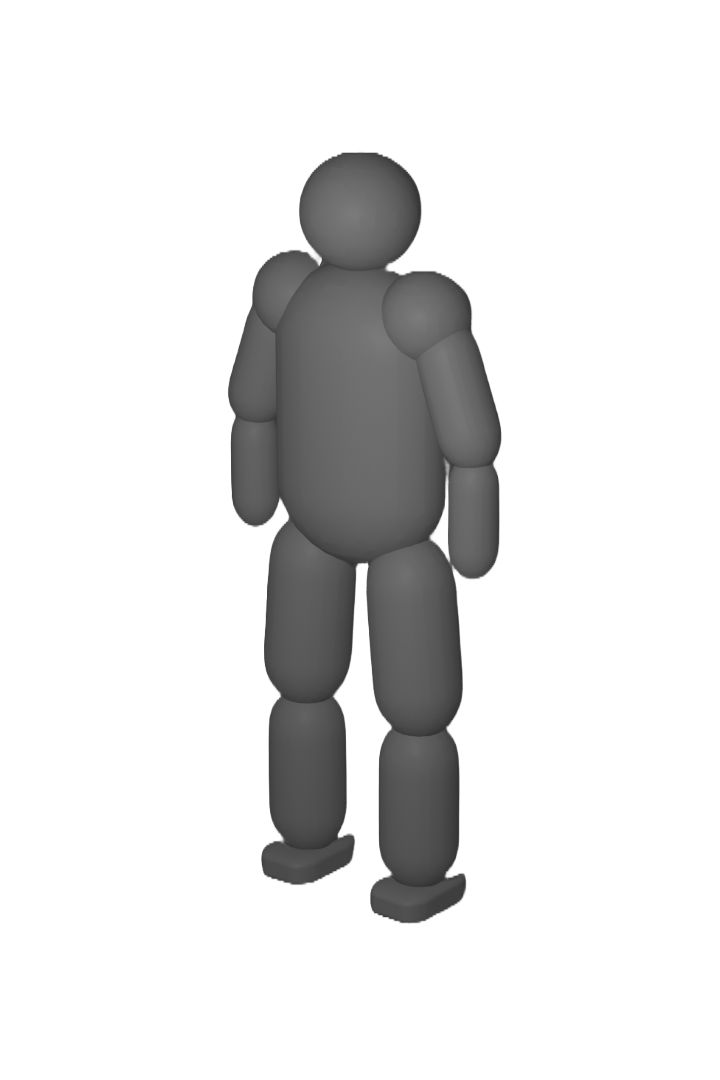
\includegraphics[scale=0.25]{visual_model.png}
    \caption{Трехмерная модель}
    \label{fig:visual_model}
  \end{minipage}
\hfill
  \begin{minipage}[t]{0.475\textwidth}
    \centering
    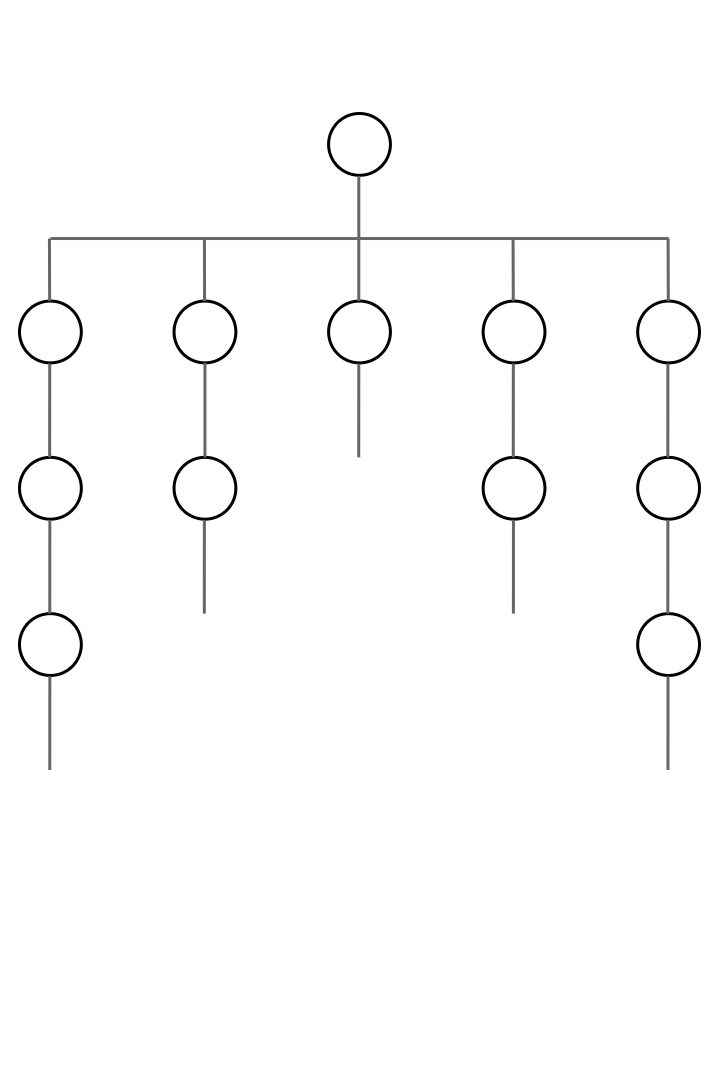
\includegraphics[scale=0.25]{kinematic_tree.png}
    \caption{Кинематическое дерево. Круги обозначают шарниры, а соединения между кругами -- твердые тела}
    \label{fig:kinematic_tree}
  \end{minipage}
\end{figure}

Кинематическое дерево -- это система из $n$ твердых тел, соединенных между собой $m$ шарнирами. Каждый из шарниров, кроме корневого, ограничивает относительное движение тел, которые он соединяет. Например, призматический шарнир оставляет только поступательное движение вдоль выбранной оси. Корневой шарнир, в свою очередь, определяет возможность системы перемещаться в пространстве и бывает двух видов: плавающий, то есть не накладывающий ограничений, и фиксирующий.

Для того чтобы приводить в движение отдельные тела, некоторые шарниры могут быть снабжены приводами, которые генерируют необходимые силы и моменты сил. В таком случае шарнир называется активным, иначе, соответственно, неактивным. Отметим, что корневой шарнир обычно остается без привода. Таким образом за движение системы как целого отвечает сила трения, что сохраняет физическую корректность, но сильно усложняет управление кинематическим деревом.

В данной работе персонаж моделируется как кинематическое дерево, все шарниры которого имеют привод, причем силы и моменты сил, генерируемые в корневом шарнире, минимизируются в оптимизаторе. Такая модель в большинстве ситуаций эквивалентна кинематическому дереву с неактивным корневым шарниром, однако оставляет возможность нарушить физическую корректность при необходимости. На рисунках \ref{fig:visual_model} и \ref{fig:kinematic_tree} изображен пример трехмерной модели персонажа и соответствующего кинематического дерева.

\subsubsection{Обобщенные координаты}

При работе с кинематическим дерево важную роль играет способ, выбранный для описания положения и ориентации тел в пространстве, поскольку он во многом определят простоту, устойчивость и вычислительную сложность моделирования. Основные способы -- это максимальные координаты и обобщенные координаты.

Максимальные координаты описывают тела по отдельности, используя по 6 чисел на каждое, а ограничения, накладываемые шарнирами, учитывают при решении уравнения динамики. Такой способ позволяет использовать существующие системы физического моделирования, но страдает от ошибок работы с вещественными числами, которые приводят к тому, что тела открепляются друг от друга.

Обобщенные координаты, напротив, учитывают связи между телами. Например, для кинематического дерева, состоящего из двух тел, соединенных вращательным шарниром, используется 7 чисел, первые 6 из которых описывают положение и ориентацию одного из тел, а оставшееся -- угол поворота вокруг оси шарнира. Такой способ минимизирует количество используемых чисел и неявно учитывает ограничения.

В данной работе используются обобщенные координаты, скорости и ускорения. Отметим, что обобщенные скорости позволяют выразить скорость любого шарнира. Для этого необходимо умножить их на якобиан шарнира. После чего можно получить скорость любой точки твердого тела, прикрепленного к шарниру, зная ее положение.

\subsubsection{Уравнение динамики}

Уравнение динамики кинематического дерева, может быть выведено из принципа наименьшего действия, и имеет вид
\begin{equation*}
  H \ddot{q} + C(q, \dot{q}) + G(q) = u + J^{T} f, \tag{1.1}\label{eq:1.1}
\end{equation*}
где $q, \dot{q}, \ddot{q}$ -- обобщенные координаты, скорости и ускорения, $H$ -- матрица инерции, $C$ -- центробежная и кориолисова силы, $G$ -- сила тяготения, $u$ -- силы и моменты сил, генерируемые приводами, $J$ -- якобиан, и $f$ -- внешние силы.

В качестве неизвестной в уравнении \ref{eq:1.1} может выступать $\ddot{q}$ или $u$. Алгоритмы, которые находят $\ddot{q}$, называются алгоритмами прямой динамики, а те, которые находят $u$, -- обратной.

Для приведения кинематического дерева в движение необходимо использование алгоритма прямой динамики. В данной работе используется алгоритм articulated rigid body, разработанный и описанный в \cite{Featherstone}, который имеет меньшую вычислительную сложностью в сравнении с остальными.

\subsubsection{Импульс и момент импульса}

В разработке систем управления персонажем активно используются такие величины как импульс и момент импульса кинематического дерева, поскольку их производные тесно связаны с положениями центра масс и центра давления (уравнения \ref{eq:1.9}, \ref{eq:1.10} и \ref{eq:1.11}), которые, в свою очередь, являются индикаторами баланса.

Напомним, что центр давления -- это точка, где можно приложить силу реакции опоры, то есть результирующую сил нормальной реакции опоры и сил трения, так чтобы момент этих сил относительно центра масс не изменился.

В \cite{OrinG} показана связь импульса и момента импульса кинематического дерева, выраженных в неподвижной системе отсчета, расположенной в центре масс, с обобщенными скоростями, имеющая следующий вид
\begin{equation*}
\begin{bmatrix} P\\ L \end{bmatrix} = A \dot{q}, \tag{1.2}\label{eq:1.2}
\end{equation*}
где $P$ -- импульс, $L$ -- момент импульса, а $A$ -- это центроидальная матрица.

Центроидальная матрица, как и матрицей инерции, является фундаментальной характеристикой кинематического дерева, которая зависит только от массы, инерции и значения обобщенных координат твердых тел, составляющих его.

При разделении центроидальной матрицы на две уравнение \ref{eq:1.2} принимает вид
\begin{align*}
  P &= A_{P} \dot{q}, \tag{1.3}\label{eq:1.3} \\
  L &= A_{L} \dot{q}. \tag{1.4}\label{eq:1.4}
\end{align*}

При дифференцировании уравнения \ref{eq:1.3} и \ref{eq:1.4} принимают вид
\begin{align*}
  \dot{P} &= \dot{A_{P}} \dot{q} + A_{P} \ddot{q}, \tag{1.5}\label{eq:1.5} \\
  \dot{L} &= \dot{A_{L}} \dot{q} + A_{P} \ddot{q}. \tag{1.6}\label{eq:1.6}
\end{align*}

Полученные уравнения \ref{eq:1.5} и \ref{eq:1.6} позволяют вычислить обобщенные ускорения необходимые чтобы производные импульса и момента импульса приняли требуемые значения, а следовательно и положения центра масс и центра давления.

% TODO: Тут бы дорисовать руки, но не хочется
\begin{figure}[ht]
  \begin{minipage}{\textwidth}
    \centering
    \begin{tikzpicture}
      % character
      \node [rectangle, minimum width = 0.7cm, minimum height = 3.0cm, draw, fill = white, rotate around = {19:(1.4, -2.1)}] at (1.4, -2.1) {};
      \node [rectangle, minimum width = 0.7cm, minimum height = 2.6cm, draw, fill = white] at (-0.4, -2.7) {};
      \node [rectangle, minimum width = 0.7cm, minimum height = 2.4cm, draw, fill = white, fill opacity = 1.0] at (-0.4, -5.2) {};
      \node [rectangle, minimum width = 0.7cm, minimum height = 2.4cm, draw, fill = white, fill opacity = 1.0] at (1.26, -5.2) {};
      \node [rectangle, minimum width = 1.5cm, minimum height = 3.0cm, draw, fill = white, fill opacity = 1.0] at (0, 0) {};

      % ground
      \draw (-2, -6.4) -- (2.8, -6.4);

      % gravity
      \filldraw [fill = black] (0.1, -0.5) circle (2pt) node [above left] {$c$};
      \draw [-{Latex[length=4mm, width=2mm]}, line width = 0.5mm] (0.1, -0.5)  -- node[left] {$mg$} (0.1, -3.0);

      % ground reaction force
      \filldraw [fill = black] (0.2, -6.4) circle (2pt) node [below right] {$p$};
      \draw [-{Latex[length=4mm, width=2mm]}, line width = 0.5mm] (0.2, -6.4) -- node[right] {$f$} (0.8, -4.4);

    \end{tikzpicture}
    \caption{Силы}
    \label{fig:forces}
  \end{minipage}
\end{figure}

Рассмотрим силы, действующие на кинематическое дерево (рисунок \ref{fig:forces}). Запишем второй закон Ньютона и основное уравнение вращательной динамики
\begin{align*}
\dot{P} &= mg + f, \tag{1.7}\label{eq:1.7} \\
\dot{L} &= (p - c) \times f, \tag{1.8}\label{eq:1.8}
\end{align*}
где $c$ -- центр масс, $p$ -- центр давления, $m$ -- суммарная масса, и $f$ -- результирующая сил нормальной реакции опоры и сил трения.

Исключая $f$ из уравнений \ref{eq:1.7} и \ref{eq:1.8}, получим
\begin{equation*}
\dot{L} = (p - c) \times (\dot{P} - mg). \tag{1.9}\label{eq:1.9}
\end{equation*}

Теперь, запишем определение импульса кинематического дерева, рассматривая его как систему твердых тел
\begin{equation*}
  P = \sum_{i = 1}^{n} m_{i} \dot{x_{i}},
\end{equation*}
где $x_{i}$, $m_{i}$ -- положения и массы. Используя следующую цепочку равенств
\begin{equation*}
  \sum_{i = 1}^{n} m_{i} \dot{x_{i}} = \frac{d}{dt} (\sum m_{i} x_{i}) = \frac{d}{dt} (mc) = m \dot{c},
\end{equation*}
преобразуем уравнение к виду
\begin{equation}
  P = m \dot{c}, \tag{1.10}\label{eq:1.10}
\end{equation}
а дифференцированием к виду
\begin{equation}
  \dot{P} = m \ddot{c}. \tag{1.11}\label{eq:1.11}
\end{equation}
